\subsection{Trilateration}
\subsection{Trilateration}
Trilateration is the technique utilized to find the co-ordinate of any point with the distance of the point given from fixed known points.	

\begin{figure}[htpb]
	\centering
	\scalebox{.5}{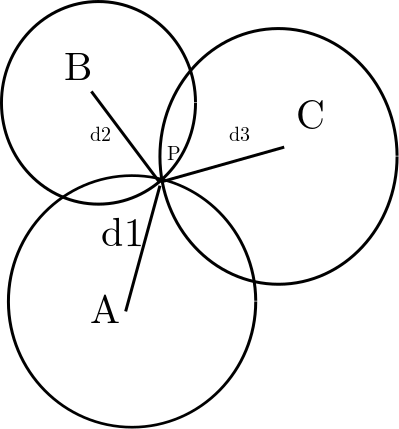
\includegraphics{./Images/Trilateration.png}}
	\caption{Trilateration}
	\label{fig:Trilateration}
\end{figure}

If in figure \ref{fig:Trilateration} the Point to be located is $P$ and the distance of $P$ from $A$, $B$ and $C$ is known respectively to be $r_1$, $r_2$, and $r_3$ to us.If we know the coordinate of the points $A(x_1,y_1,z_1)$, $B(x_2,y_2,z_2)$ and $C(x_3,y_3,z_3)$ then the coordinate $(x,y,z)$ of the point $P$ can be calculated from the set of equations:


In three dimensional geometry, when it is known that a point lies on the surfaces of three spheres, then the centers of the three spheres along with their radii provide sufficient information to narrow the possible locations down to no more than two(unless the centers lie on a straight line).

\subsubsection{Derivation}
The intersections of the surfaces of three spheres is found by formulating the equations for three sphere surfaces and then solving the three equations for three unknown $x$,$y$ and $z$.
\begin{eqnarray}
	\label{equation1} (x-x_1)^2+(y-y_1)^2+(z-z_1)^2={r_1}^2 \\
	\label{equation2} (x-x_2)^2+(y-y_2)^2+(z-z_2)^2={r_2}^2 \\
	\label{equation3} (x-x_3)^2+(y-y_3)^2+(z-z_3)^2={r_3}^2 
\end{eqnarray}

To simplify the calculations, the equations are formulated so that the centers of the spheres lie on $z=0$ plane. Also the formulation is such that location of one of the known points is origin and that of another known point is on the x-axis. Assuming this thing, we first calculate the location of the required unknown point and then the solution is transformed back to the original three dimensional Cartesian coordinate system.

Therefore, the coordinates of three known points are : $P_1(0,0,0)$, $P_2(d,0,0)$ and $P_3(i,j,0)$. Now, equation \ref{equation1}, equation \ref{equation2} and equation \ref{equation3} become :
\begin{eqnarray}
	\label{equation4}  x^2+y^2+z^2={r_1}^2 \\ 
	\label{equation5} (x-d)^2+y^2+z^2={r_2}^2 \\ 
	\label{equation6} (x-i)^2+(y-j)^2+z^2={r_3}^2 
\end{eqnarray}

Now, using $r_1$ and $r_2$ to eliminate $y$ and $z$ from equation and solving for $x$, we get
\begin{eqnarray}
\nonumber	{r_1}^2-{r_2}^2=x^2-(x-d)^2 \\ 
%\nonumber	{r_1}^2-{r_2}^2=2xd-d^2 \\ 
%\nonumber	{r_1}^2-{r_2}^2+d^2=2xd \\
	x=\frac{{r_1}^2-{r_2}^2+d^2}{2d}
\end{eqnarray}

Assuming that the first two spheres intersect in more than one point, that is,
\begin{equation}
	d-r_1<r_2<d+r1 \nonumber
\end{equation}

Now, substituting the equation for $x$ back into the equation for the first sphere produces the equation for a circle. The solution to the intersection of the first two spheres is:
\begin{equation}
y^2+z^2={r_1}^2-\frac{({r_1}^2-{r_2}^2+d^2)^2}{4d^2} \nonumber
\end{equation}

Substituting the value of $z^2$ from equation \ref{equation4}, we get, 
\begin{equation}
y=\frac{{r_1}^2-{r_3}^2+i^2+j^2}{2j}-\frac{i}{j}x
\end{equation}
Now that the $x$ and $y$ coordinates of the solution points are determined, the formula can be rearranged for the first sphere to find the z-coordinate of the solution point. Therefore,
\begin{equation}
	z=\pm \sqrt{{r_1}^2-x^2-y^2}
\end{equation}

Now the solution to all three points x, y and z is found. Because z is expressed as the positive or negative square root, it is possible for there to be zero, one or two solutions to the problem.

This last part can be visualized as taking the circle found from intersecting the first and second sphere and intersecting that with the third sphere. If that circle falls entirely outside of the sphere, z is equal to the square root of a negative number, which implies no real solution exists. If that circle touches the sphere on exactly one point, z is equal to zero. If that circle touches the surface of the sphere at two points, then z is equal to plus or minus the square root of a positive number.

\subsection{Final Computation}

The Derivation section pointed out that the coordinate system in which the sphere centers are designated must be such that
\begin{enumerate}
	\item All three centers are in the plane $z=0$
	\item The sphere center, $P_1$, is at the origin
	\item The sphere center, $P_2$, is on the x-axis.
\end{enumerate}
In general the problem will not be given in a form such that these requirements are met.

This problem can be overcome as described below where the points, $P_1$, $P_2$, and $P_3$ are treated as vectors from the origin where indicated. $P_1$, $P_2$, and $P_3$ are expressed in the original coordinate system.

The unit vector in the direction from $P_1$ to $P_2$ is:
\begin{equation}
\hat e_x = \frac{ P_2 - P_1 }{ \| P_2 - P_1 \| } \nonumber
\end{equation}

The signed magnitude of the x component, of the vector from $P_1$ to $P_3$ is:
\begin{equation}
i = \hat e_x \cdot ( P_3 - P_1 )  \nonumber
\end{equation}
The unit vector in the y direction can be found as:
\begin{equation}
\hat e_y = \frac{ P_3 - P_1 - i \; \hat e_x}{ \| P_3 - P_1 - i \; \hat e_x \| } \nonumber
\end{equation}
The third basis unit vector is 
\begin{equation}
\hat e_z = \hat e_x \times \hat e_y \nonumber
\end{equation}
Therefore, \\
The distance between the centers $P_1$ and $P_2$ is $d = \| P_2 - P_1 \|$  and the signed magnitude of the y component,of the vector from $P_1$ to $P_3$ is:
\begin{equation}
j = \hat e_y \cdot ( P_3 - P_1 ) \nonumber
\end{equation}


Using $i, \;  d$ and $j$ as computed above, the values for x, y and z can be solved as described in the Derivation section.Then,
\begin{equation}
	\vec p_{1,2} = P_1 + x \ \hat e_x + y \ \hat e_y \ \pm \ z \ \hat e_z
	\label{OriginalSolution}
\end{equation}
Equation \ref{OriginalSolution} gives the points in the original coordinate system, since, $\hat e_x, \; \hat e_y$ and $\hat e_z$, the basis unit vectors, are expressed in the original coordinate system.
